
%%%%%%%%%%%%%%%%%%%%%%% file typeinst.tex %%%%%%%%%%%%%%%%%%%%%%%%%
%
% Author: Mauricio Matamoros
% Updated: July 3, 2017
% Contact: mauricio@robocupathome.org
%
% This is the LaTeX source for the TDPTemplate using
% the LaTeX document class 'llncs.cls' Springer LNAI format
% used in the RoboCup Symposium submissions.
% http://www.springer.com/computer/lncs?SGWID=0-164-6-793341-0
%
% It may be used as a template for your own TDP - copy it
% to a new file with a new name and use it as the basis
% for your Team Description Paper
%
% NB: the document class 'llncs' has its own and detailed documentation, see
% ftp://ftp.springer.de/data/pubftp/pub/tex/latex/llncs/latex2e/llncsdoc.pdf
%
% Remark: Last page with specs won't be included in Camera ready TDP's.
%
%%%%%%%%%%%%%%%%%%%%%%%%%%%%%%%%%%%%%%%%%%%%%%%%%%%%%%%%%%%%%%%%%%%

\documentclass[runningheads,a4paper]{llncs}
\usepackage{amssymb}
\setcounter{tocdepth}{3}
\usepackage{graphicx}
\usepackage{amssymb}
\usepackage[utf8]{inputenc}
\usepackage[hidelinks]{hyperref}
\usepackage{url}
\usepackage{float}
\usepackage{amsmath}
\usepackage{graphicx}
\usepackage{wrapfig}
\usepackage{fancyhdr}
\usepackage{titling}
\usepackage{xcolor}
\usepackage{lipsum}
\newcommand{\robospecs}{%
	\newpage%
	\pagenumbering{gobble}%
	\pagestyle{fancy}%
	\fancyhf{}%
	\chead{$|$}
	\rhead{\footnotesize Robot Description}%
	\lhead{\footnotesize Tech United Eindhoven}%
	\rfoot{Robot software and hardware specification sheet}%
}

\newcommand{\BnL}[1][1em]{ 
\includegraphics[width=#1]{images/bnl.jpg} } 


%%%%%%%%%%%%%%%%%%%%%%%%%%%%%%%%%%%%%%%%%%%%%%%%%%%%%%%%%%%%%%%%%%%%%%%%%%%%%%%%%%%%
%
% Title
%
%%%%%%%%%%%%%%%%%%%%%%%%%%%%%%%%%%%%%%%%%%%%%%%%%%%%%%%%%%%%%%%%%%%%%%%%%%%%%%%%%%%%
\title{Lipsum 2018 Team Description Paper}

\author{Main-author \and Co-author \and Team Members}
\institute{Affiliation name and address, \\
\texttt{http://devoted-web-site.url}}


\begin{document}
\maketitle

%%%%%%%%%%%%%%%%%%%%%%%%%%%%%%%%%%%%%%%%%%%%%%%%%%%%%%%%%%%%%%%%%%%%%%%%%%%%%%%%%%%%
%
% Abstract
%
%%%%%%%%%%%%%%%%%%%%%%%%%%%%%%%%%%%%%%%%%%%%%%%%%%%%%%%%%%%%%%%%%%%%%%%%%%%%%%%%%%%%

\begin{abstract}

In your abstract, please state your main research line and your achievements of this year (on which problem or set of problems are you focusing all the team efforts). Tell why this research is important, how are you approaching to the problem solution and which results do you expect to obtain.

\end{abstract}


%%%%%%%%%%%%%%%%%%%%%%%%%%%%%%%%%%%%%%%%%%%%%%%%%%%%%%%%%%%%%%%%%%%%%%%%%%%%%%%%%%%%

\section{Introduction}
A Team Description Paper (hereinafter referred as TDP) is an 8-pages long scientific paper, detailing information on the technical and scientific approach of the team's research.

The present document is a template for the TDPs as they should be presented in 2018. An updated version of this template can be download from \\\url{https://github.com/RoboCupAtHome/TDPTemplate}.


\section{TDP contents}
While writing the TDP, focus on your current research, clearly stating all scientific contribution, and why are they important for you and the league. The length of the TDP is limited to 8 pages including references. Exceeding the number of pages will automatically void your application.

Although reviewers share a common background in the domain of service robotics, is very unlikely that they are actively involved in your research field. The organizing committee kindly asks authors to keep this in mind and write in a more descriptive and less analytic way. The main goal of a TDP is tell others about your latest practical achievement, how your team managed to solve the problem, what strategy was chosen and why, while at the same time trying to convince your reader that what you are doing is useful or applicable in a daily life scenario.

The Team Description Paper shall use the \textit{Springer LNAI format}\footnotemark used in the RoboCup Symposium submissions, and has a hard limit of 8 pages without altering margins or spacing (including references but excluding the annex). Please notice that changes to the margins, space between paragraphs, and font size are not allowed (such TDP will be rejected). We suggest to leave the hardware and software description for the end of the paper in the annex.\footnotetext{\url{http://www.springer.com/computer/lncs?SGWID=0-164-6-793341-0}}

\textbf{Important Notice:} Attaching to the requested format is important for the camera ready version of the TDPs can be included in the memories of the competition.

Remember that the TDP must contain the following information:

\begin{itemize}
	\item Innovative technology and scientific contribution
	\item Focus of research/research interests
	\item Re-usability of the system for other research groups
	\item Applicability of the robot in the real world
	\item \textbf{DSPL \& SSPL:} When the robot depicted in the TDP or Team Video is different from the league's standard one, the TDP must clearly state how the addressed approach and described software will be adapted to the standard platform robot.
\end{itemize}

\textbf{Remark:} The language for the TDP body, its graphics, tables, images, and all additional content must be English. Content in other languages must be translated.

\subsection{TDP Annex}
The TDP's Robot Description Annex is an appendix of arbitrary length that should be attached at the end of the TDP and summarizes the robot's software and hardware technical specifications.

When present, the annex must contain the following information:

\begin{itemize}
	\item Photo(s) of the robot
	\item \textbf{OPL only:} Brief, compact description of the robot's hardware.
	\item \textbf{DSPL \& SSPL:} Please skip hardware description.
	\item Brief, compact description of the robot's software (including commercial products, freeware, Open Source, etc.).
	\item List of all external computing devices and the software running on them.
	\item List of all cloud computing resources intended to be used.
	\item Brief, compact description of all external devices (e.g. smart home devices, transceivers, helper robots, etc.).
\end{itemize}

Examples are provided at the end of this document in
\hyperlink{page.9}{page~9~(DSPL)},
\hyperlink{page.10}{page~10~(OPL)}, and
\hyperlink{page.11}{page~11~(SSPL)}.

\textbf{Copyright note:} All TDPs sent for qualification may be made publicly available in the RoboCup @Home Wiki for further reference. On submitting, teams implicitly grant permission to RoboCup @Home and the RoboCup Federation to copy, distribute, upload, publish, and use the manuscript to promote the event and the league at convenience.

\section{Background}
% We are Buy n Large. We have no competitors so no background is required.
\lipsum[1-3]

\section{BnL Trash Seeker Algorithm (Main research)}
\lipsum[4-10]

\section{BnL All-purpose Speech Recognizer (Main research)}
\lipsum[11-13]

\section{Other relevant contributions}
\lipsum[14]
\subsection{Dirt Detector Algorithm}
\lipsum[15-17]
\subsection{Green Plant Seeker Algorithm}
\lipsum[18-20]
\subsection{Trash Seeker Algorithm}
\lipsum[20-22]

\section{Experiments and results}
\lipsum[23-24]

\section{Conclusions and future work}
\lipsum[25-26]

%%%%%%%%%%%%%%%%%%%%%%%%%%%%%%%%%%%%%%%%%%%%%%%%%%%%%%%%%%%%%%%%%%%%%%%%%%%%%%%%%%%%
%
% Bibliography
%
%%%%%%%%%%%%%%%%%%%%%%%%%%%%%%%%%%%%%%%%%%%%%%%%%%%%%%%%%%%%%%%%%%%%%%%%%%%%%%%%%%%%

\bibliographystyle{unsrt}
\bibliography{bibliography}

{\vfill\begin{center}\huge\color{red}TDP must \textbf{NOT} exceed 8 pages\end{center}}

%%%%%%%%%%%%%%%%%%%%%%%%%%%%%%%%%%%%%%%%%%%%%%%%%%%%%%%%%%%%%%%%%%%%%%%%%%%%%%%%%%%%
%
% Robot Specifications
%
%%%%%%%%%%%%%%%%%%%%%%%%%%%%%%%%%%%%%%%%%%%%%%%%%%%%%%%%%%%%%%%%%%%%%%%%%%%%%%%%%%%%

\robospecs
\section*{HSR's Software and External Devices}
% In this section briefly describe the software and hardware of the robot

\setlength\intextsep{0pt}
\begin{wrapfigure}[5]{r}{0.3\textwidth}
	\centering
	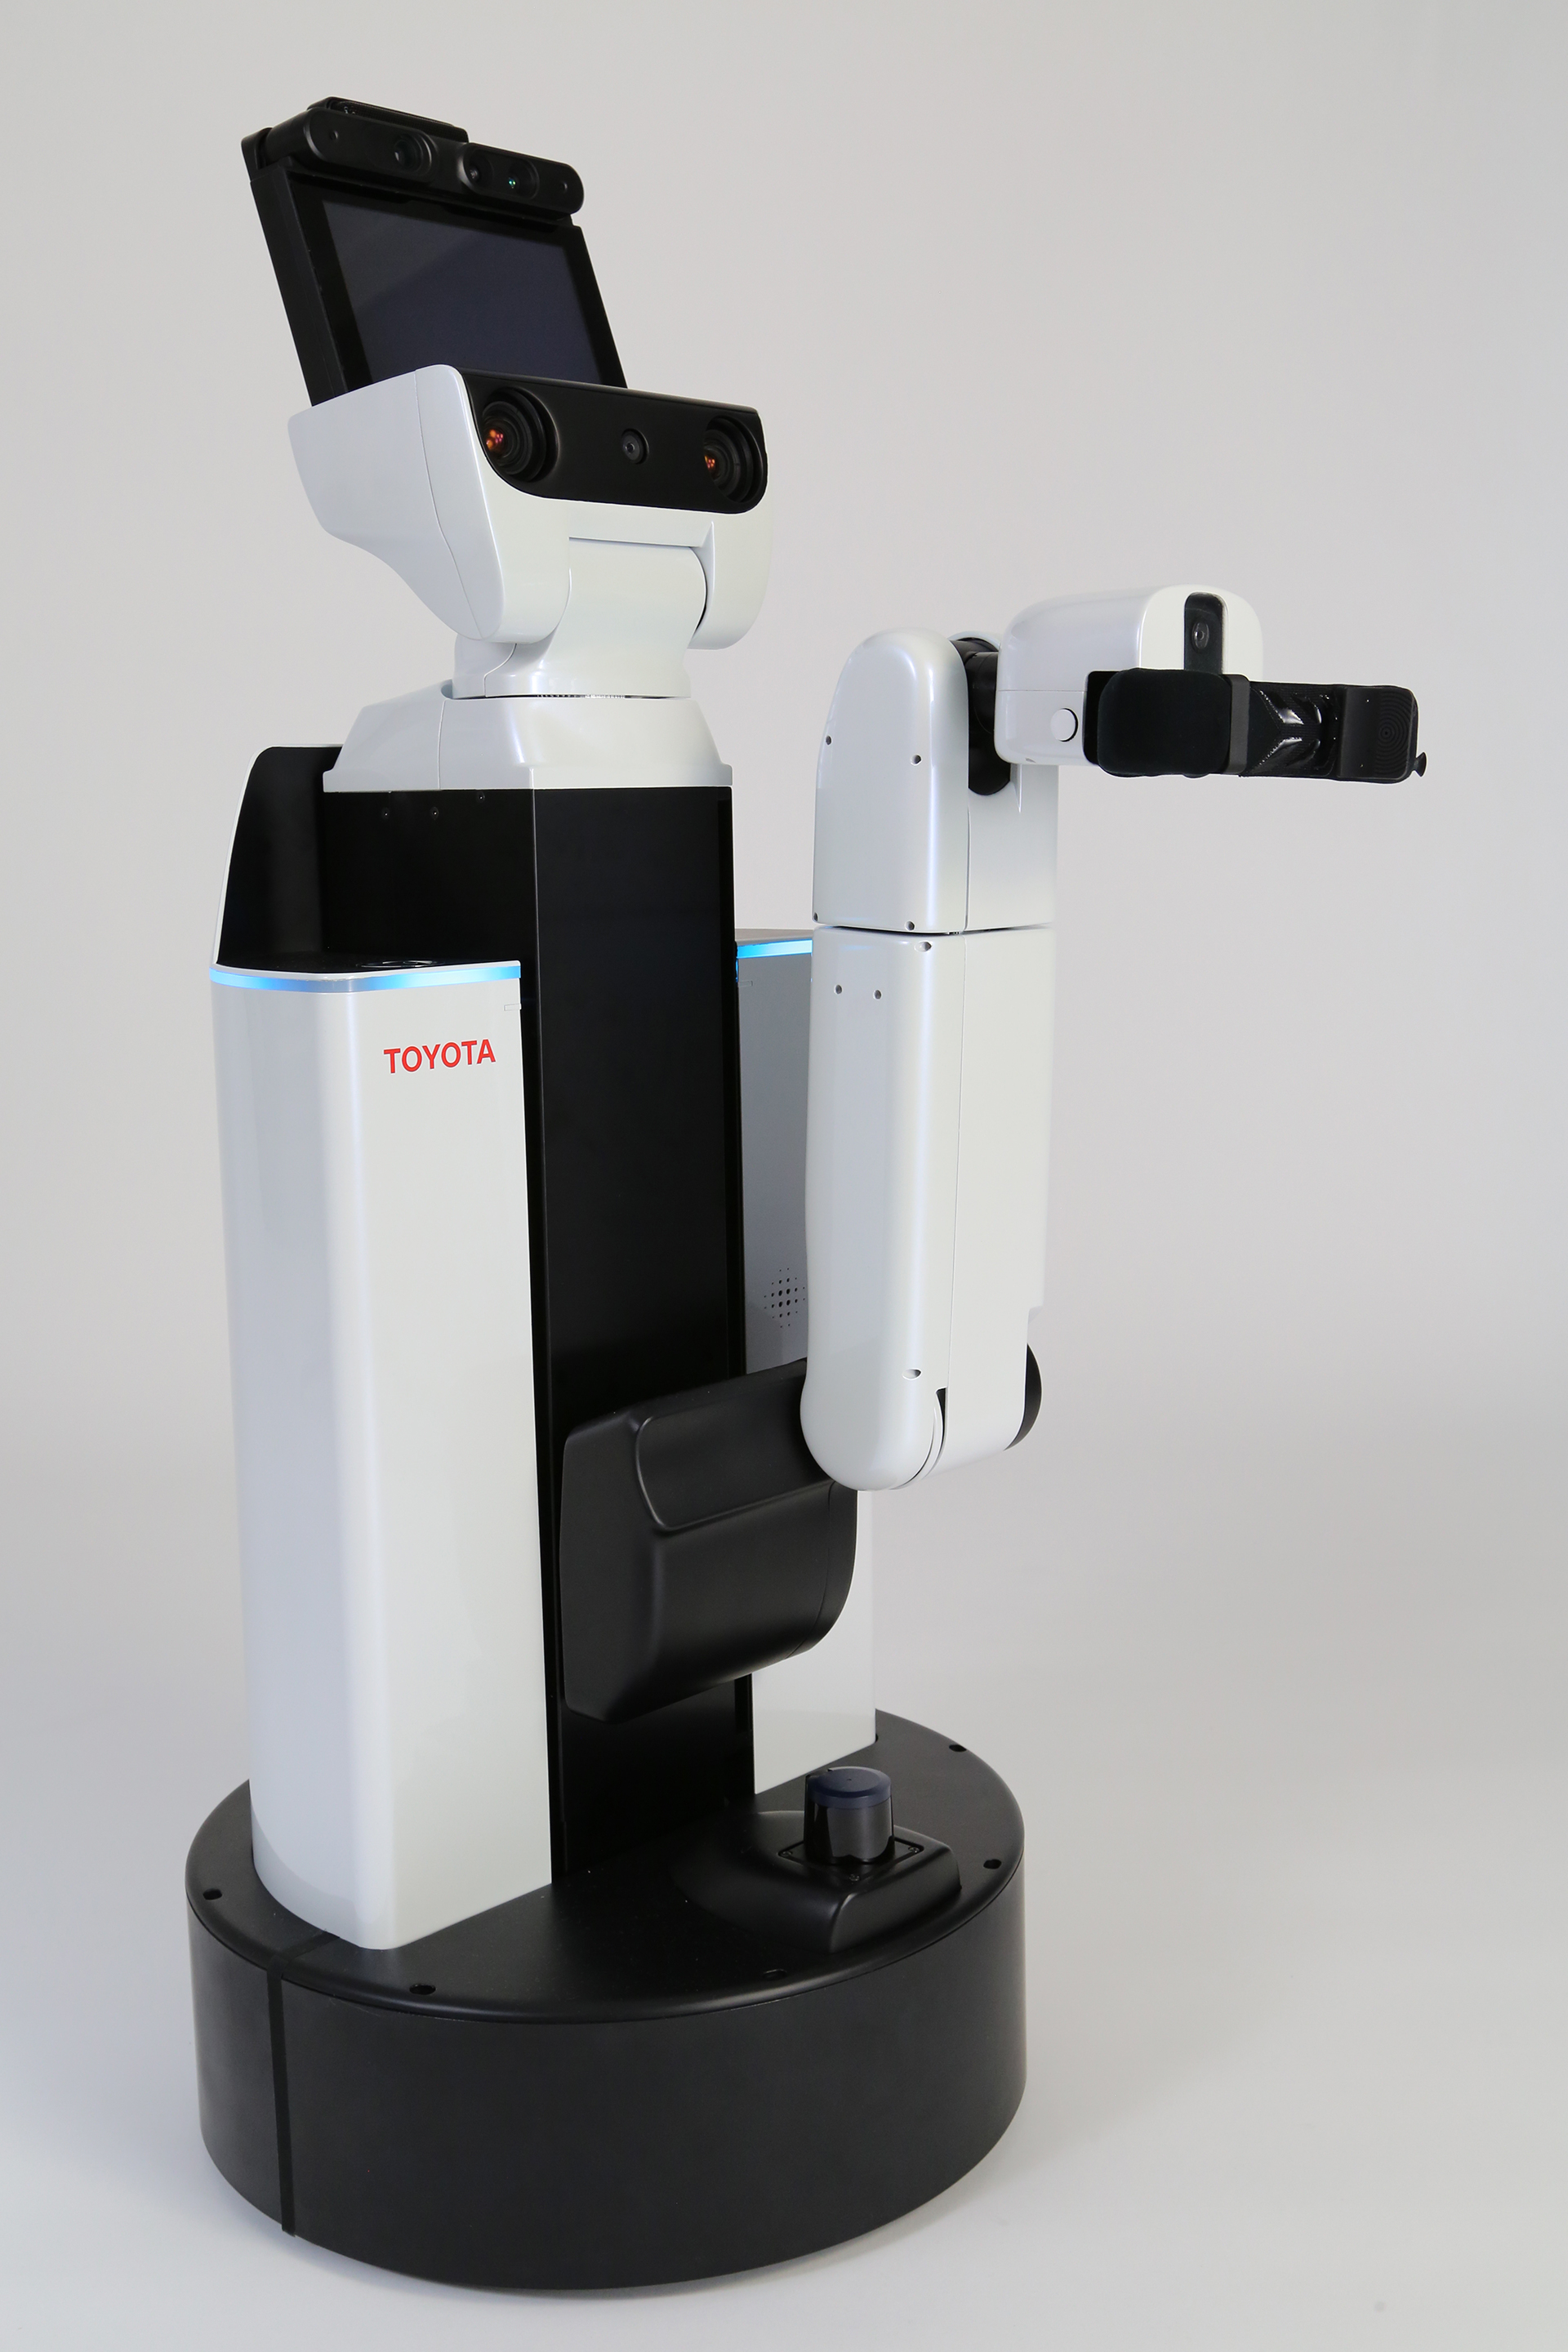
\includegraphics[width=0.3\textwidth]{Toyota_HSR}
	\caption{The Toyota HSR Robot, HERO}
	\label{fig:hsr}
\end{wrapfigure}

We use a standard \textit{Toyota} HSR robot unit. To differentiate our unit, we named it HERO. We wanted to link the name to our AMIGO and SERGIO domestic service robots.

\section*{HERO's Software Description}
% Please describe in this section the software you are using to control your robot. Consider the following example:

An overview of the software used by the Tech United Eindhoven @Home robots can be found in Table~\ref{tab:softwarespec}.
All our software is developed open-source at GitHub\footnote{\url{https://github.com/tue-robotics}}.
\\\newline
Currently, we have some \textit{image\_recognition} packages released into the current ROS Kinetic distribution and can be installed with use of \textit{apt}.

\begin{table}[H]
    \begin{center}
    \caption{Software overview of the robots.}
    \label{tab:softwarespec}
    %\vspace{-0.1cm}
    \renewcommand{\arraystretch}{1.0}
    \setlength{\tabcolsep}{5pt}
        \begin{tabular}{p{0.3\textwidth} p{0.7\textwidth}}
            \toprule
            Operating system & Ubuntu 16.04 LTS Server\\

            Middleware & ROS Kinetic~\cite{Quigley2009}\\

            Low-level control software & Orocos Real-Time Toolkit~\cite{Bruyninckx2001}\newline
            \url{https://github.com/tue-robotics/rtt_control_components}
            \\

            Simulation & Custom kinematics + sensor simulator \newline
            \url{https://github.com/tue-robotics/fast_simulator}
            \\

            World model & \acrfull{ed}, custom \newline
            \url{https://github.com/tue-robotics/ed}\\

            Localization & Monte Carlo~\cite{Fox2003} using \gls{ed}, custom \newline \url{https://github.com/tue-robotics/ed\_localization}\\

            SLAM & Gmapping package \newline \url{http://wiki.ros.org/gmapping}\\

            Navigation & CB Base navigation
            \newline
            \url{https://github.com/tue-robotics/cb_base_navigation}
            \newline
            Global: custom A* planner\newline Local: modified ROS DWA~\cite{Fox1997}\\

            Arm navigation & Custom implementation using MoveIt and Orocos KDL\newline
            \url{https://github.com/tue-robotics/tue_manipulation}
            \\

            Object recognition & Tensorflow ROS \newline
			\url{https://github.com/tue-robotics/image\_recognition/tree/master/tensorflow\_ros}\\

            People detection & Custom implementation using contour matching \newline
            \url{https://github.com/tue-robotics/ed_perception}
            \\
            Face detection \& recognition & Openface ROS \newline \url{https://github.com/tue-robotics/image\_recognition/tree/master/openface\_ros} \\

            Speech recognition & Julius Speech Recognition \newline
            \url{https://github.com/julius-speech/julius}\\
            Speech synthesis & Toyota\texttrademark \hspace{0em} Text-to-Speech\\
            Task executors & SMACH \newline
            \url{https://github.com/tue-robotics/tue_robocup}\\
            \bottomrule
        \end{tabular}
    \end{center}
\end{table}

This our current software implementation on our robots AMIGO and SERGIO, which participate in the open league. Because of the pending delivery of the Toyota HSR and related documentation, we are not able to provide the specific software implementation. As described in our selection qualification paper, our goal is to use the same software as possible on all our robots, including the Toyota HSR.

\section*{External Devices}
% Please describe in this section the external devices used by your robot. Consider the following example:

\textit{HERO relies on the following external hardware:}

\begin{itemize}
	\item Mother-ship
	\item Data Cluster
	\item $3 \times$ Ultra-Power laptops.
\end{itemize}

\section*{Cloud Services}
% Please describe in this section the Cloud Services and online software used by your robot. Consider the following example:

\textit{HERO connects the following cloud services:}
\begin{itemize}
	\item Localization and mapping: Geolocalization system.
	\item Navigation: Navigator
	\item Speech recognition: All-purpose recognizer.
\end{itemize} 
\newpage
\section*{Amigo's Hardware Description}
% In this section briefly describe the software and hardware of the robot

\setlength\intextsep{0pt}
\begin{wrapfigure}[15]{r}{0.3\textwidth}
	\centering
	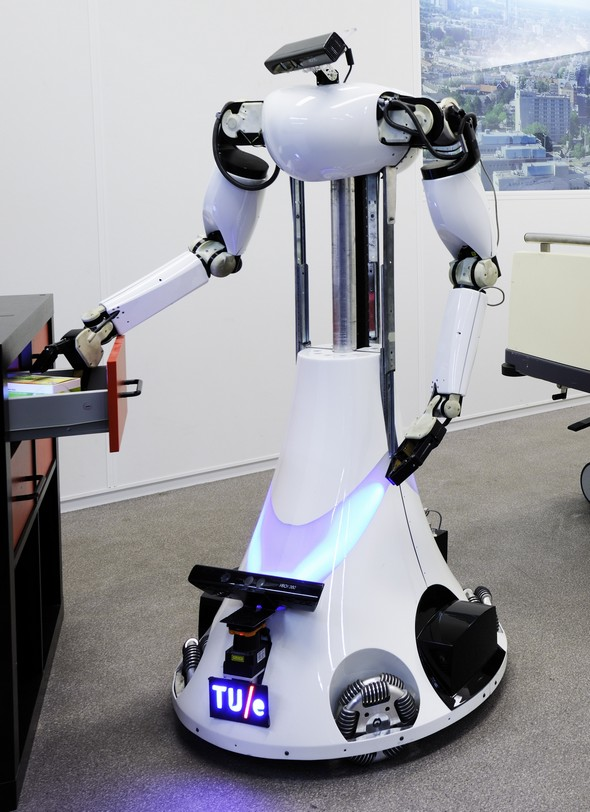
\includegraphics[width=0.3\textwidth]{amigo}
	\caption{The Amigo Robot}
	\label{fig:amigo}
\end{wrapfigure}

AMIGO (Autonomous Mate for Intelligent Operations, see Fig.~\ref{fig:amigo}) has competed in RoboCup@Home since 2011. Its design is based on a Middle Size League soccer robot, equipped with two Philips\texttrademark \hspace{0em} Experimental Robotic Arms mounted on an extensible upper body. Based on our experiences with AMIGO, SERGIO (Second Edition Robot for Generic Indoor Operations, has been developed. The main differences with AMIGO are the use of Mecanum wheels which are compliantly suspended, the torso with two degrees of freedom and the modular setup. The core specifications of AMIGO are shown in Table~\ref{tab:hardwarespec}. More details about the robots are on the Robotic Open Platform\footnote{\texttt{http://www.roboticopenplatform.org/}}, where all CAD drawings, electrical schematics and CAD files are published. SERGIO will not enter the competition this year. \\

\begin{table}[H]
    \begin{center}
    \caption{Core specifications of AMIGO}
    \label{tab:hardwarespec}
    \renewcommand{\arraystretch}{1.0}
    \setlength{\tabcolsep}{5pt}
        \begin{tabular}{p{0.2\textwidth} p{0.4\textwidth}}
            \toprule
            & AMIGO \\
            \midrule
            Name & Autonomous Mate for IntelliGent Operations \\
            Base & Fully holonomic omni-wheel platform  \\
            Torso & 1 vertical DoF using a ball screw \\
            Manipulators & 2 7-DoF Philips\texttrademark \hspace{0em} Experimental Robotic Arms \\
            Neck & Pan-tilt unit using two Dynamixel RX-64 servo actuators \\
            Head & Microsoft Kinect\texttrademark \hspace{0em} for XBox 360\texttrademark \\
            External devices & Wireless emergency button \\
            Dimensions & Diameter: $0.75\ \mathrm{m}$, height: $\pm1.5\ \mathrm{m}$ \\
            Weight & $\pm84\ \mathrm{kg}$ \\
            Additional sensors & Hokuyo UTM-30LX laser range finder on base and torso\\
            Microphone & R{\O}DE Videomic and Matrix Creator\\
            Batteries & $4\times$ Makita $24\ \mathrm{V},\ 3.3\ \mathrm{Ah}$ \\
            Computers & $3\times$ AOpen Mini PC with Core-i7 processor and $8\ \mathrm{GB}$ RAM and NVidia Jetson TX2 \\
            \bottomrule
        \end{tabular}
    \end{center}
\end{table}

\newpage
\section*{Amigo's Software Description}
% Please describe in this section the software you are using to control your robot. Consider the following example:

An overview of the software used by the Tech United Eindhoven @Home robots is shown in Table~\ref{tab:softwarespec}.
All our software is developed open-source on GitHub\footnote{\url{https://github.com/tue-robotics}}.
\\\newline
Some \textit{image\_recognition} packages are released into the ROS Kinetic distribution and can be installed with use of \textit{apt}.\\


\begin{table}[H]
    \begin{center}
    \caption{Software overview of Amigo.}
    \label{tab:softwarespec}
    %\vspace{-0.1cm}
    \renewcommand{\arraystretch}{1.0}
    \setlength{\tabcolsep}{5pt}
        \begin{tabular}{p{0.3\textwidth} p{0.7\textwidth}}
            \toprule
            Operating system & Ubuntu 16.04 LTS Server\\

            Middleware & ROS Kinetic~\cite{Quigley2009}\\

            Low-level control software & Orocos Real-Time Toolkit~\cite{Bruyninckx2001}\newline
            \url{https://github.com/tue-robotics/rtt_control_components}
            \\

            Simulation & Custom kinematics + sensor simulator \newline
            \url{https://github.com/tue-robotics/fast_simulator}
            \\

            World model & \acrfull{ed}, custom \newline
            \url{https://github.com/tue-robotics/ed}\\

            Localization & Monte Carlo~\cite{Fox2003} using \gls{ed}, custom \newline \url{https://github.com/tue-robotics/ed_localization}\\

            SLAM & Gmapping package \newline \url{http://wiki.ros.org/gmapping}\\

            Navigation & CB Base navigation
            \newline
            \url{https://github.com/tue-robotics/cb_base_navigation}
            \newline
            Global: custom A* planner\newline Local: modified ROS DWA~\cite{Fox1997}\\

            Arm navigation & Custom implementation using MoveIt and Orocos KDL\newline
            \url{https://github.com/tue-robotics/tue_manipulation}
            \\

            Object recognition & Tensorflow ROS \newline
			\url{https://github.com/tue-robotics/image_recognition/tree/master/tensorflow_ros}\\

            People detection & Custom implementation using contour matching \newline
            \url{https://github.com/tue-robotics/ed_perception}
            \\
            Face detection \& recognition & Openface ROS \newline \url{https://github.com/tue-robotics/image_recognition/tree/master/openface_ros} \\

            Speech recognition & Dragonfly + Windows\texttrademark \hspace{0em} Speech Recognition \newline
            \url{https://github.com/tue-robotics/dragonfly_speech_recognition}\\
            Speech synthesis & \texttrademark \hspace{0em} Text-to-Speech\\
            Task executors & SMACH \newline
            \url{https://github.com/tue-robotics/tue_robocup}\\
            \bottomrule
        \end{tabular}
    \end{center}
\end{table}

\section*{External Devices}
% Please describe in this section the external devices used by your robot. Consider the following example:
TODO: Update this page!\\

\textit{Amigo relies on the following external hardware:}

\begin{itemize}
	\item  Wireless emergency stop
	\item  etc.
\end{itemize}

\section*{Cloud Services}
% Please describe in this section the Cloud Services and online software used by your robot. Consider the following example:

\textit{Amigo connects the following cloud services:}
\begin{itemize}
	\item Localization and mapping:
    \item Speech recognition:
    \item etc.
\end{itemize} 
\newpage
\section*{HSR's Software and External Devices}
% In this section briefly describe the software and hardware of the robot

\setlength\intextsep{0pt}
\begin{wrapfigure}[5]{r}{0.3\textwidth}
	\centering
	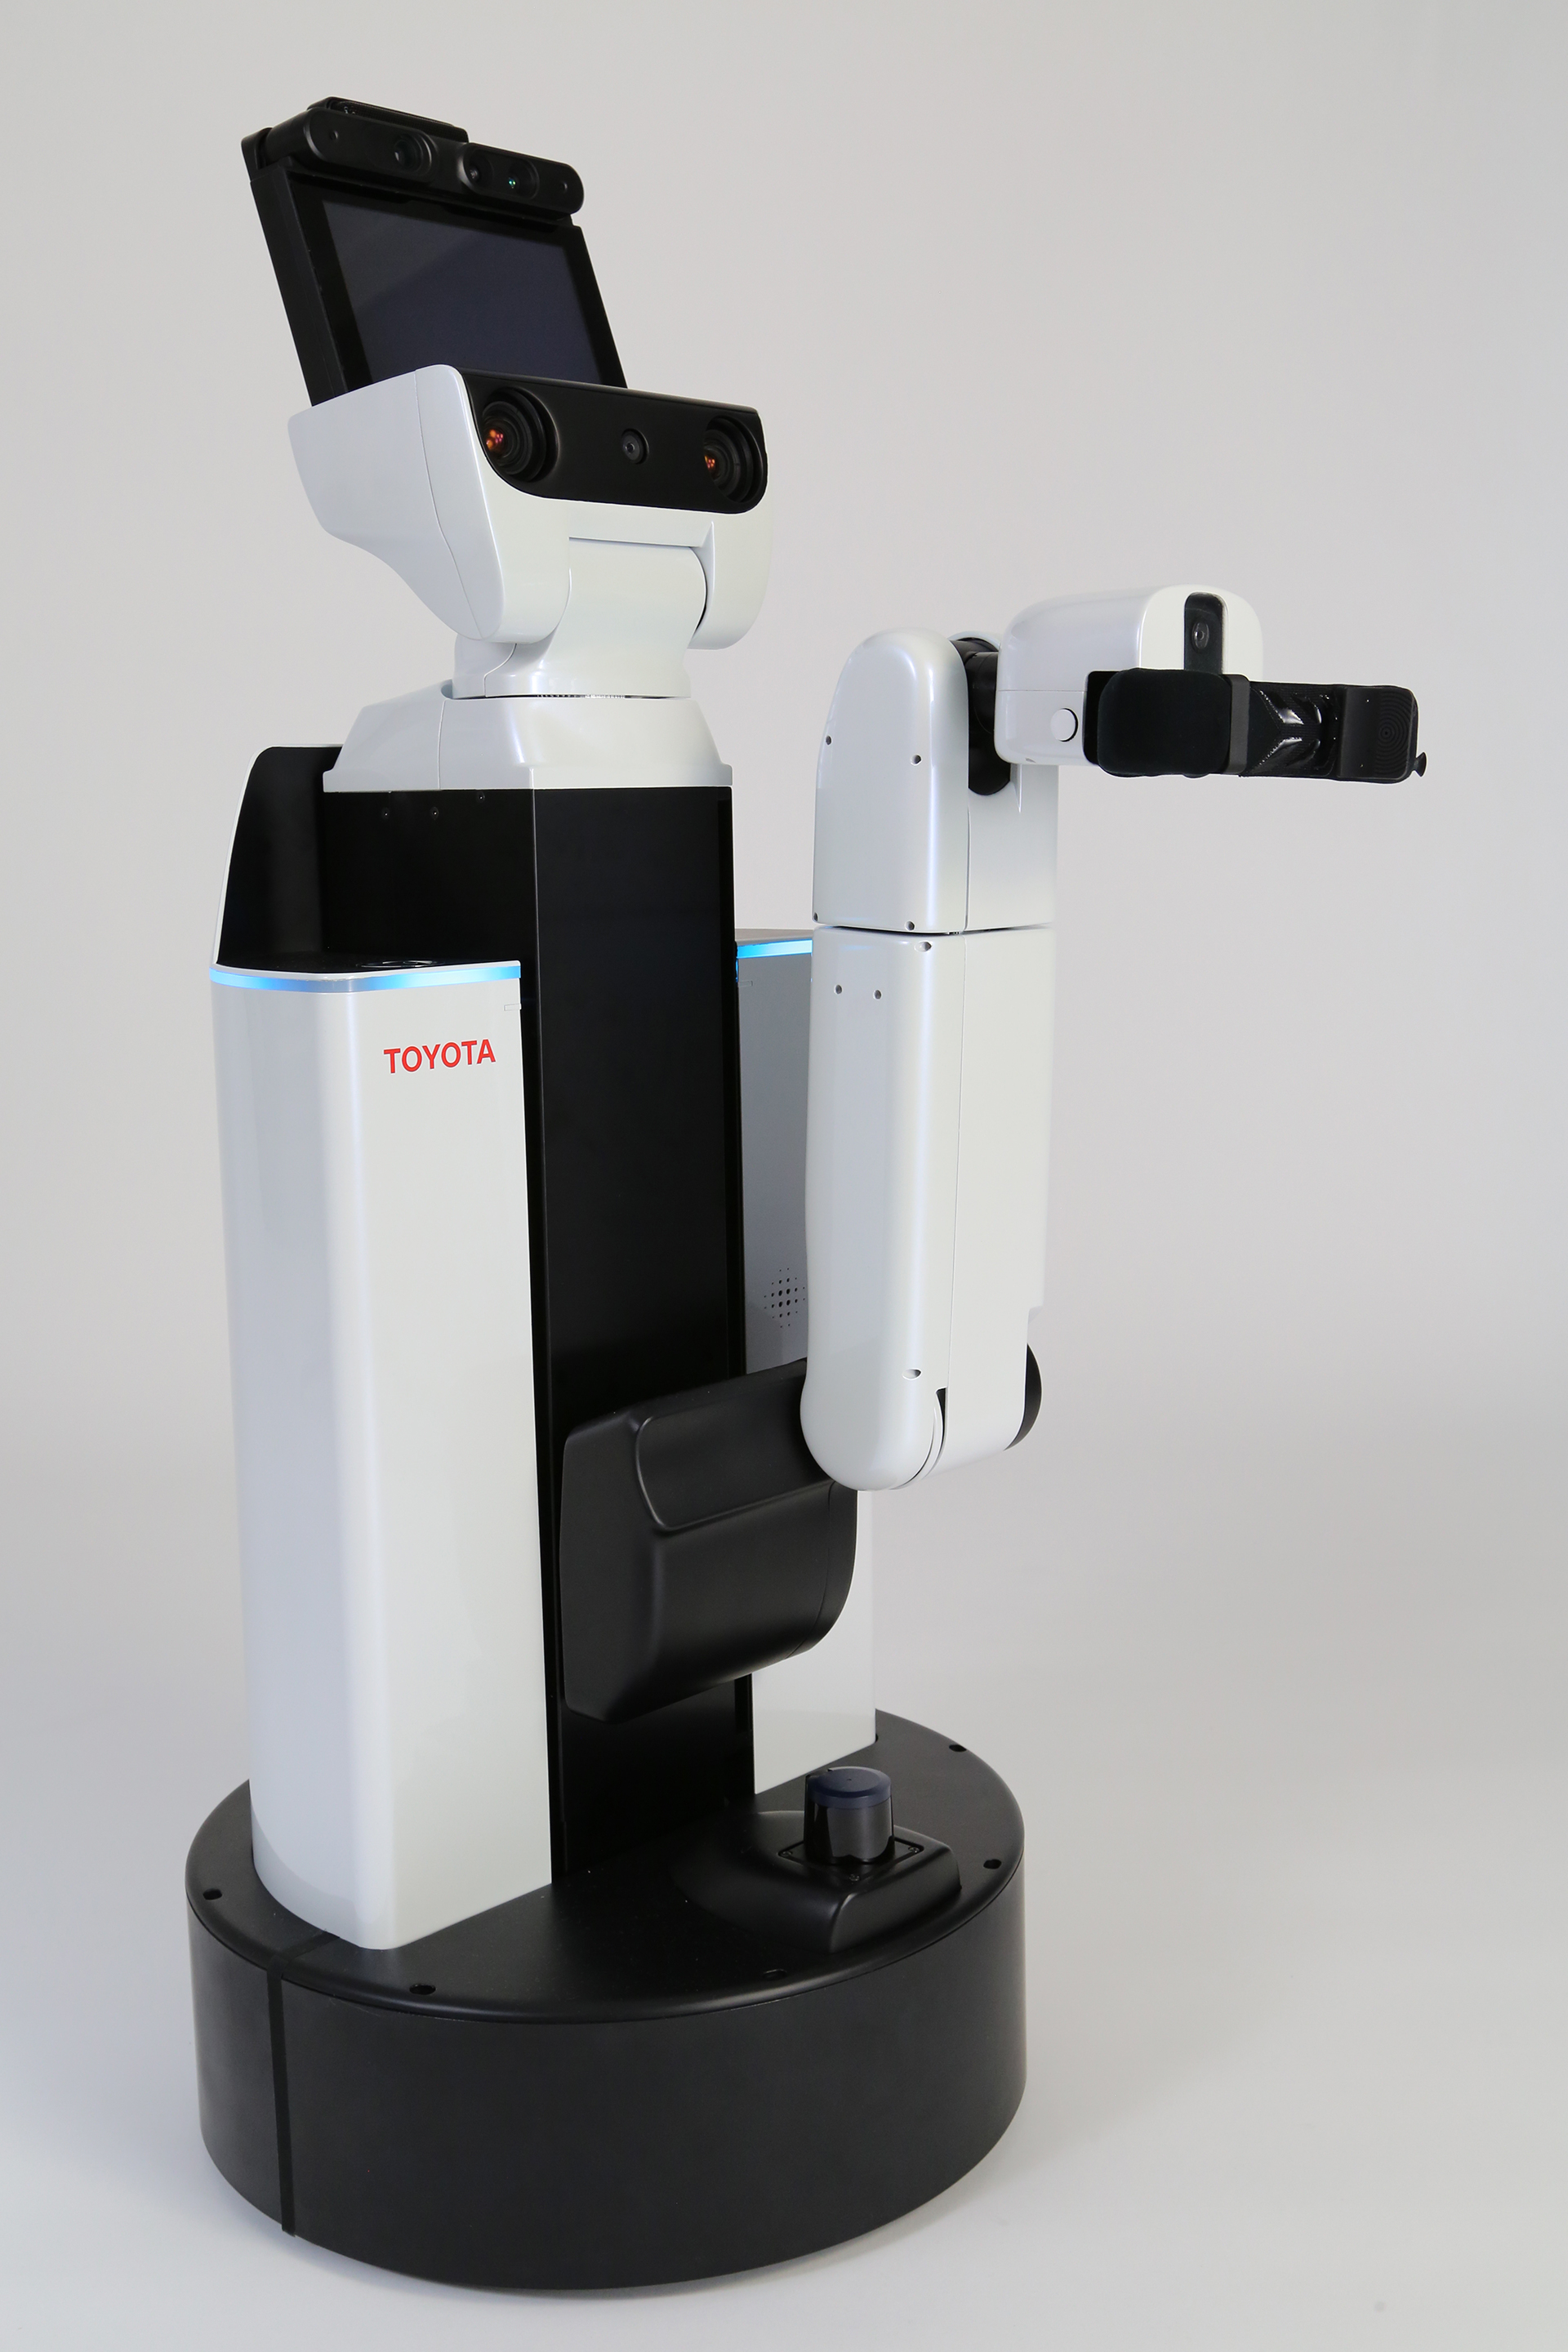
\includegraphics[width=0.3\textwidth]{Toyota_HSR}
	\caption{The Toyota HSR Robot, HERO}
	\label{fig:hsr}
\end{wrapfigure}

We use a standard \textit{Toyota} HSR robot unit. To differentiate our unit, we named it HERO. We wanted to link the name to our AMIGO and SERGIO domestic service robots.

\section*{HERO's Software Description}
% Please describe in this section the software you are using to control your robot. Consider the following example:

An overview of the software used by the Tech United Eindhoven @Home robots can be found in Table~\ref{tab:softwarespec}.
All our software is developed open-source at GitHub\footnote{\url{https://github.com/tue-robotics}}.
\\\newline
Currently, we have some \textit{image\_recognition} packages released into the current ROS Kinetic distribution and can be installed with use of \textit{apt}.

\begin{table}[H]
    \begin{center}
    \caption{Software overview of the robots.}
    \label{tab:softwarespec}
    %\vspace{-0.1cm}
    \renewcommand{\arraystretch}{1.0}
    \setlength{\tabcolsep}{5pt}
        \begin{tabular}{p{0.3\textwidth} p{0.7\textwidth}}
            \toprule
            Operating system & Ubuntu 16.04 LTS Server\\

            Middleware & ROS Kinetic~\cite{Quigley2009}\\

            Low-level control software & Orocos Real-Time Toolkit~\cite{Bruyninckx2001}\newline
            \url{https://github.com/tue-robotics/rtt_control_components}
            \\

            Simulation & Custom kinematics + sensor simulator \newline
            \url{https://github.com/tue-robotics/fast_simulator}
            \\

            World model & \acrfull{ed}, custom \newline
            \url{https://github.com/tue-robotics/ed}\\

            Localization & Monte Carlo~\cite{Fox2003} using \gls{ed}, custom \newline \url{https://github.com/tue-robotics/ed\_localization}\\

            SLAM & Gmapping package \newline \url{http://wiki.ros.org/gmapping}\\

            Navigation & CB Base navigation
            \newline
            \url{https://github.com/tue-robotics/cb_base_navigation}
            \newline
            Global: custom A* planner\newline Local: modified ROS DWA~\cite{Fox1997}\\

            Arm navigation & Custom implementation using MoveIt and Orocos KDL\newline
            \url{https://github.com/tue-robotics/tue_manipulation}
            \\

            Object recognition & Tensorflow ROS \newline
			\url{https://github.com/tue-robotics/image\_recognition/tree/master/tensorflow\_ros}\\

            People detection & Custom implementation using contour matching \newline
            \url{https://github.com/tue-robotics/ed_perception}
            \\
            Face detection \& recognition & Openface ROS \newline \url{https://github.com/tue-robotics/image\_recognition/tree/master/openface\_ros} \\

            Speech recognition & Julius Speech Recognition \newline
            \url{https://github.com/julius-speech/julius}\\
            Speech synthesis & Toyota\texttrademark \hspace{0em} Text-to-Speech\\
            Task executors & SMACH \newline
            \url{https://github.com/tue-robotics/tue_robocup}\\
            \bottomrule
        \end{tabular}
    \end{center}
\end{table}

This our current software implementation on our robots AMIGO and SERGIO, which participate in the open league. Because of the pending delivery of the Toyota HSR and related documentation, we are not able to provide the specific software implementation. As described in our selection qualification paper, our goal is to use the same software as possible on all our robots, including the Toyota HSR.

\section*{External Devices}
% Please describe in this section the external devices used by your robot. Consider the following example:

\textit{HERO relies on the following external hardware:}

\begin{itemize}
	\item Mother-ship
	\item Data Cluster
	\item $3 \times$ Ultra-Power laptops.
\end{itemize}

\section*{Cloud Services}
% Please describe in this section the Cloud Services and online software used by your robot. Consider the following example:

\textit{HERO connects the following cloud services:}
\begin{itemize}
	\item Localization and mapping: Geolocalization system.
	\item Navigation: Navigator
	\item Speech recognition: All-purpose recognizer.
\end{itemize} 

\nocite{*}

\end{document}
